%!TEX root = main.tex
% \begin{figure}[htb]
% \begin{center}
% %optional pour enlever un peu d'espace blanc de votre silhouette
% %\vspace{-.3cm}
%  %\includegraphics[keepaspectratio,width=0.5\textwidth]{fig/nomde}
% % analoog
% %\vspace{-0.6cm}
%  % \caption{ici un logo}
%  % \label{fig:ruglogo}
% %analoog
% %\vspace{-.6cm}
% \end{center}
% \end{figure}

% Utilisation du template
% \cite(reference à citer)
% \ref(figure à référencer)

%\bibliography{reference}

\chapter{Generative Adversarial Networks}

\paragraph{}
	La première partie de cette étude nous a permis de maîtriser l'utilisation de réseaux en perceptron et de structurer une architecture logicielle efficace et souple pour l'étude des GAN. \\
	Après avoir obtenu des résultats satisfaisants dans la classification de motifs sur la base MNIST, nous étudions la génération de données à l'aide de réseaux de neurones en nous basant sur le concept de GAN, introduit par I. Goodfellow en 2016 \cite{goodfellow_generative_2014}.\\
	Notre objectif dans cette partie est d’appréhender le concept de GAN et de l'appliquer sur notre programme afin d'étudier les différents paramètres. 
\section{Principe}
	\paragraph{}
		Le GAN s'inscrit dans les problèmes de générations de données par ordinateur. Ses modèles cherchent à produire de données nouvelles respectant un certain nombre de contraintes. Les applications possibles sont très nombreuses tant au niveau scientifique qu'industriel, avec, par exemple, la modélisation de nouvelles protéines, le dessin de circuits intégrés, etc. 
		Le but de nos GAN sera de générer des images que l’on ne pourra distinguer de « vraies » images, prises avec un appareil photo.\\

		Le principe général est le suivant : \\ un GAN est constitué de deux réseaux de neurones, le Générateur (G) et le Discriminateur (D). Le Générateur a pour but de créer les images et le Discriminateur de déterminer si les images qu’on lui donne sont de « vraies » images ou ont été créées par le Générateur. Ces deux réseaux sont mis en compétition : le Générateur a pour but de tromper le Discriminateur tandis que le Discriminateur doit détecter les « fausses » images.\\
		L’apprentissage du Discriminateur se fait à la fois sur des images générées par le Générateur et de « vraies » images, issues d’une banque d’images afin de continuellement améliorer sa capacité de discernement.\\
		L’apprentissage du Générateur dépend de la réponse du  Discriminateur : lorsqu’il génère une image, on la donne au Discriminateur pour voir si le Générateur a réussi à le tromper. Le discriminateur sert donc de fonction d'erreur au Générateur.
	
\begin{figure}[h]
  \centerline{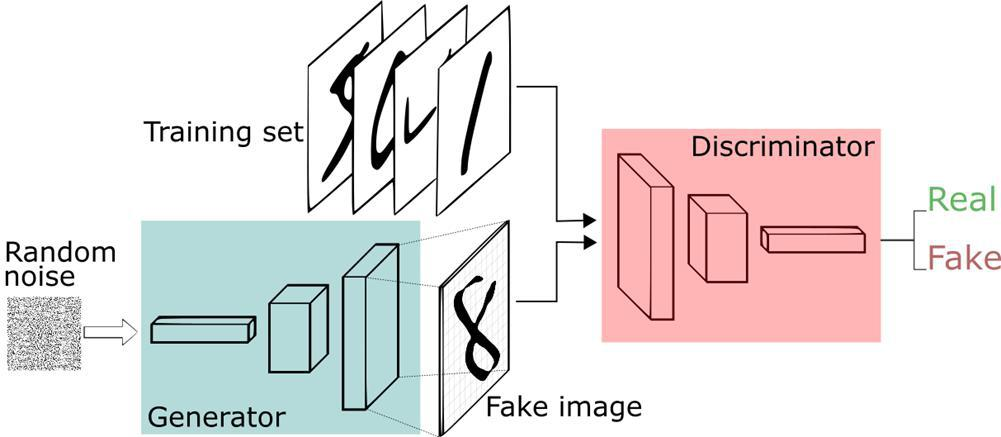
\includegraphics[width=0.6\linewidth]{fig/conceptGAN.png}}
  \caption{Fonctionnement du GAN}
  \label{fig:concept_gan}
\end{figure}

	\paragraph{}
		De façon plus formelle, on travaille avec 3 distributions : $p_x$, la distribution idéale des vraies images, $p_{data}$, la distribution de l'échantillon des vraies images et $p_{model}$ la distribution réalisée par les images issues du Générateur. Le but de l’apprentissage est de rapprocher $p_{model}$ de $p_x$. Comme $p_x$ nous est inconnu, on va plutôt s'approcher de $p_{data}$.\\
		On dispose de deux fonctions de coûts $J_D(\theta_G, \theta_D)$ et $J_G(\theta_G, \theta_D)$, représentant respectivement les fonctions de coûts du Discriminateur et du Générateur. On note $\theta_G$ et $\theta_D$ les paramètres des réseaux. Les fonctions de coûts dépendent bien des paramètres des deux réseaux car le Discriminateur apprend à discerner les vraies images des fausses, dépendantes du générateur, et le générateur apprend via le résultat du Discriminateur.\\ C'est un problème d'optimisation simultanée. 
		Il peut également être décrit comme un problème de jeux à informations complètes. G a accès aux données de D, mais ne peut influer que sur $\theta_G$ et D a accès aux données de G, mais ne peut influer que sur $\theta_D$. Cette vision permet de déduire un algorithme où chaque joueur va faire un mouvement de manière optimal, afin de tendre vers un équilibre de Nash.

\section{Apprentissage}

	\paragraph{}
		L’apprentissage consiste à appliquer cette méthode de jeu à l'apprentissage des réseaux de neurones.
		Nous fournissons au Discriminateur des images $x$ (de la BDD MNIST par exemple) et lui demandons de nous renvoyer un réel entre 0 et 1, qui représente son degré de confiance sur le fait que l’image fournie ait été tirée d’une banque de données authentiques ou du Générateur. Les réponses attendues sont respectivement ($D(x) = 1$) et ($D(x) =0$) ce qui nous permet de calculer des erreurs pour la descente de gradient du Discriminateur.\\ 
		Le Générateur, quant à lui, génère une image à partir d’un vecteur de bruit $z$. Cette image est ensuite jugée par le Discriminateur : $D(G(z)) = 1$ si le Générateur a dupé le Discriminateur et 0 sinon. L'objectif du Générateur est d'être le plus proche possible de la première situation, l'erreur pour la descente du gradient du Générateur en est déduite.\\
		L'apprentissage complet se fait en alternant les 2 phases successivement, chaque réseau jouant tour à tour. On parle de réseau concurrent car le Discriminateur cherche à obtenir $D(G(z)) = 0 $ pour tout $z$ et le Générateur $D(G(z)) = 1$.

	\paragraph*{Problèmes liés à la convergence}
		L'apprentissage des GANs n'est pas simple à maîtriser car ils ne fonctionnent pas comme un seul réseau qui apprend avec une algorithme de descente de gradients. Il s'agit en réalité d'une descente de gradient simultanée ($J_G \text{ et } J_D$) qui n'est pas un cas particulier, mais une généralisation du problème classique d'optimisation. La résolution mathématique de ce problème n'est pas triviale, et les méthodes ne s'adaptent pas facilement aux réseaux de neurones. La méthode proposée ci-dessous est donc une heuristique que l'on peut fortement adapter. Elle a fait ses preuves dans de nombreux cas, malgré son manque d’appui mathématique. Cependant d'autres façons de voir les choses permettent d'obtenir des résultats toujours corrects mais avec une plus grande rigueur. Les questionnements mathématiques seront abordés dans les axes de recherches.  

\section{Paramètres des GANS}

	Voici une description des paramètres principaux sur lesquels on peut jouer pour l'implémentation d'un GAN. Ils sont nombreux car la description précédente est en réalité peu restrictive.

	\begin{itemize}
	 	\item Fonctions de coûts
	 	\item Ratios d'apprentissage
	 	\item Paramètres classiques des réseaux de neurones (Structures des réseaux, pas d'apprentissage, etc.)
	\end{itemize}


\section{Structure et utilisation du code}
	{description des modifications importantes pour le GAN (or optimisation du code source)}


\section{Premiers résultats pour des GANs simples}
	Afin d'appréhender correctement le fonctionnement des GANs, il est nécessaire de tester de nombreux paramètres. Les résultats, fructueux ou non, permettent d'évaluer l'intérêt des paramètres et de comprendre le sens "physique" de leur influence.\\
	Ces essais se feront sur la base MNIST, c'est-à-dire que notre objectif sera d'obtenir des chiffres manuscrits dessinés par le générateur. Plus précisément, on attend du générateur après apprentissage que chaque entrée génère un chiffre entre 0 et 9 qu'un être humain ne peut distinguer d'un chiffre manuscrit écrit par un humain (donc de la base MNIST).

	\subsection{Méthodologie initiale}
		L'un des objectifs de ce projet est de décortiquer au mieux la méthode GAN. Pour cela, nous utilisons les réseaux de neurones les plus simples, ils seront complexifiés par la suite. La plupart des articles sur le sujet présentent des réseaux utilisant des structures avancées (couche convolutive, optimiseur de descente, etc.). Il n'est donc pas possible de se référer aux paramètres de ces articles pour obtenir immédiatement des résultats et s'assurer que notre programme tourne correctement. \\
		Pour le choix du réseau Discriminateur, le choix se porte sur des structures ayant eu de bonnes performances pour le MNIST, c'est-à-dire soit un très bon taux final, soit une vitesse de convergence élevée. En effet, le Discriminateur n'est qu'un simple classificateur sur la base MNIST. Le choix du générateur est plus complexe car il faut que la structure soit assez puissante pour dessiner des chiffres. Cela semble bien plus difficile que simplement les reconnaitre, car ils peuvent être reconnus à l'aide de features très particuliers, tandis que la génération exige une information complète. La première idée pour dimensionner le réseau est d'avoir une entrée suffisante pour générer la diversité de sortie souhaitée, mais pas nécessairement plus pour ne pas avoir un réseau trop lourd en calcul.\\
		Pour les autres paramètres, nous n'avons a priori pas d'idée précise de leurs ordres de grandeur nécessaires, en particulier pour le pas d'apprentissage (très différents pour MNIST et XOR par exemple).\\
		Nous avons donc balayé les paramètres possibles afin d'obtenir le maximum d'information avec des GANs simples.\\
		Le principal souci que nous avons eu avec cette approche fut l'évaluation des performances de nos GANs, au début de l'étude. En effet, nous n'arrivions pas encore à former des chiffres satisfaisants et, par conséquent, n'avions aucun moyen pour savoir si un paramètre était meilleur qu'un autre. \\
		Nous avons considéré l'étude de l'évolution des scores que le Discriminateur attribuait aux images de Mnist et à celles du Générateur, mais elles se sont révélées inexploitables : le score brut ne permettait pas de rendre compte de l'apprentissage effectué jusqu'alors. Et le score ne révélait en rien la qualité de l'image. 
{ici des exemples de courbes sur lesquelles on travaillait au début } 




\section{Mode Collapse}
	\subsection{Présentation du problème}
		Le problème du Mode Collapse est bien connu dans la confections de GANs. Il se traduit par un générateur qui ne produit plus qu'un type de données particulier, sans diversité. 
		Imaginons un générateur qui doit générer deux types de données : X et Y. Après quelques apprentissages, il réussit à générer des X suffisament convaincants pour tromper le Discriminateur. A ce moment, le Générateur est "récompensé" pour tromper Le Discriminateur, et ce dernier n'arrive plus à distinguer les X de la BBD de ceux générés artificiellement. Du coup le Discriminateur ne fait plus confiance aux X qu'il reçoit et se concentre sur les Y, sur lesquels il se fait davantage récompenser pour son travail. Après quelques apprentisasges à nouveau, le générateur oublie les X et se met à générer des Y trompeurs.
		Ainsi, notre GAN fournit alternativement des X et des Y médiocres sur une longue periode, alors qu'au contraire on souhaiterai obtenir des données diverses. Si ce problème est dû au fait que les données à générer sont différentes, on voit que paradoxalement, plus il y a de diversité dans les données à générer ,  moins le Collapse est important.
		
\begin{figure}[h]
  \centerline{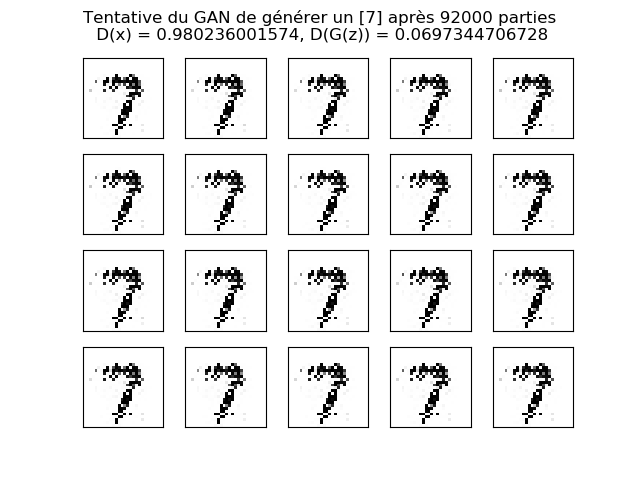
\includegraphics[width=0.6\linewidth]{fig/excollapse.png}}
  \caption{Exemple de Collapse}
  \label{fig:ex_collapse}
\end{figure}

	\subsection{Une première idée de résolution du problème}
		Une première étape pour éviter le problème est décrite dans l'article de NIPS 2014 de I.Goodfellow \cite{goodfellow_generative_2014}. Il s'agit d'ajouter du bruit sur une couche intermédiaire du Générateur. En forçant ainsi une part d'aléatoire dans le Générateur, on peut espérer qu'il ne se "verrouille" pas et ne produise qu'une donnée particulière. 
		Nous avons implémenté cette solution lors de notre travail sur MNIST. Goodfellow suggère plusieurs techniques d'implémentations : ajouter un bruit à la sortie d'une couche, multiplier le vecteur de sortie terme à terme avec un vecteur de bruit, ou encore concaténer le vecteur de sortie avec un vecteur de bruit gaussien. Nous avons choisi d'implémenter cette dernière solution. On pourrait toujours craindre que, dans le pire des cas, le Générateur décide d'attribuer au bruit des poids nuls ou négligeables. Mais lors de l'implémentation, on a néanmoins remarqué une baisse significative du taux de Mode Collapse dans nos expériences.

En figure \ref{fig:resultat_gan_bb}, on voit les résultats d'un GAN avec du bruit et un biais non nul en dernière couche. Les chiffres sont peu satisfaisants mais le réseau ne tombe pas en mode Collapse. En revanche, le dernier biais est très influent : il dessine presque à lui tout seul les 7 du réseau.
\begin{figure}[h!]
  \centering
  \begin{subfigure}[b]{.7\linewidth}
    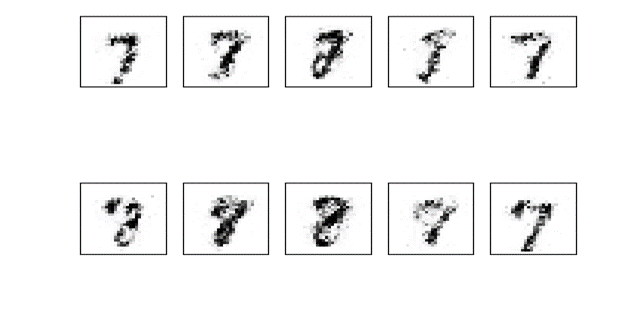
\includegraphics[width=\linewidth]{fig/resultatganbetb.png}
    \caption{Résultats d'un GAN en mettant du bruit et du biais en dernière couche}
  \end{subfigure}
  \quad
  \begin{subfigure}[b]{.2\linewidth}
    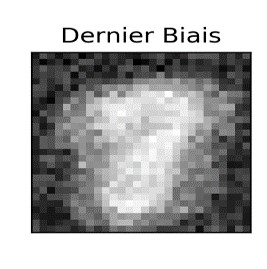
\includegraphics[width=\linewidth]{fig/resultatganbetbdernierbiais.jpg}
    \caption{Biais en dernière couche}
  \end{subfigure}
  \caption{Résultats d'un GAN apprenant sur des 7 et des 8 uniquement}
  \label{fig:resultat_gan_bb}
\end{figure}

En retirant le biais, on obtient des résultats comme à la figure \ref{fig:resultat_gan_bruit_sans_biais}. Le réseau arrive à tracer des 8 différents et même des 7 que l'on reconnaît clairement.

\begin{figure}[h!]
  \centering
  \begin{subfigure}[b]{\linewidth}
    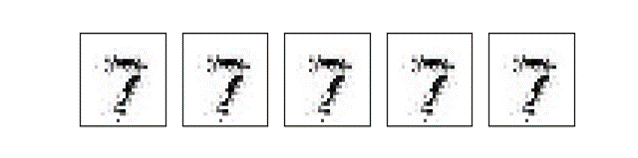
\includegraphics[width=\linewidth]{fig/resultatgannibruitnibiais7.png}
    \caption{Le GAN apprend sur des 7}
  \end{subfigure}
  \quad
  \begin{subfigure}[b]{\linewidth}
    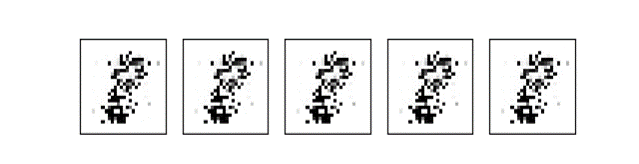
\includegraphics[width=\linewidth]{fig/resultatgannibruitnibiais8.png}
    \caption{Le GAN apprend sur des 8}
  \end{subfigure}
  \caption{Résultats d'un GAN sans bruit ni biais sur la dernière couche}
  \label{fig:resultat_gan_bruit_sans_biais}
\end{figure}

Enfin, pour un GAN sans biais ni bruit sur la dernière couche, on obtient des résultats semblables à la figure \ref{fig:resultat_gan_ni_bruit_ni_biais}. Sans bruit, ni biais, on retombe dans le monde collapse. Comme première solution, rajouter du bruit sur la dernière couche est efficace !

\begin{figure}[h]
  \centerline{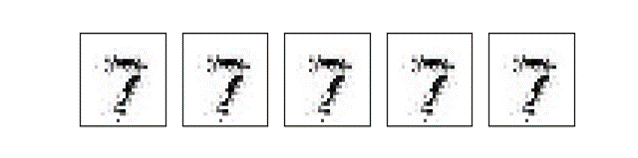
\includegraphics[width=0.6\linewidth]{fig/resultatgannibruitnibiais.png}}
  \caption{Réseau ayant appris sur des 7 et des 8, sans bruit ni biais sur la dernière couche}
  \label{fig:resultat_gan_ni_bruit_ni_biais}
\end{figure}

		\subsection{Perturber le GAN avec des "secousses" } 
		Une approche pour empêcher le GAN de tomber en Mode Collapse fut suggérée par T. Salimans. Elle consiste à ajouter une part d'aléatoire dans le processus. \\
	Plutôt que de s'attendre à ce que le Discriminateur renvoie 1 sur une image de la base de données, on calcule l'erreur à partir d'un réel proche de 1 (entre 0.7 et 0.99) afin de plus facilement le récompenser. \\
	En parallèle, de temps en temps (un cas sur deux cent, grand maximum ) on trompe le Discriminateur en lui disant qu'on attendait une vraie image lorsqu'il en traite une fausse et inversement. \\
	Ces deux techniques permettraient, en théorie, de renforcer le générateur de manière subtile (pour la première ) et de le perturber suffisamment pour sortir des situations de Collapse (deuxième technique).\\
	Cependant, les expériences menées par nos soins sur ces techniques ne se sont pas montrées concluantes, le Collapse apparaissait parfois plus vite que sans ces techniques . \\
	Cela est sans doute dû au fait que nos GANs, contrairement à ceux de Goodfellow et Salimans, n'étaient pas assez robustes pour qu'on puisse se permettre d'ajouter cette part d'aléatoire. 
	
	

	\subsection{Une autre piste : le minibatch}
		Une autre méthode destinée à empêcher le Mode Collapse et à forcer la diversité des données générées fut proposée par T.Salilmans et I.Goodfellow dans Improved techniques for training GANs \cite{salimans_improved_2016}.\\
		L'idée consiste en proposant au Discriminateur non plus une seule donnée du Générateur mais bien tout un petit paquet (minibatch). Une distance mathématique entre chacune des données de ce minibatch est calculée et traitée (passée à l'exponentielle négative) puis ajoutée à la sortie d'une couche intermédiaire du Discriminateur. \\
		Ainsi, on envoie $n$ images dans notre Discriminateur, qui possèdera sur une couche intermédiaire $n$ neurones supplémentaires, l'activation du neurone $i$ correspond à un score de ressemblance entre la donnée traitée actuellement et la donnée $i$. Le Discriminateur a donc un moyen de déterminer si les données générées par le Générateur sont toutes semblables entre elles ou non. Il pourra ainsi facilement punir le Discriminateur si celui tombait en Mode Collapse . \\
		
	



\section{Résultat sans collapse}
Ici, des résultats obtenus sans Collapse, la solution choisie fut celle qui consistait à mettre du bruit dans les couches intermédiaires. De plus, comme pour prouver que plus de diversité signifiait moins de Collapse, on s'est aperçu que le réseau avait plus de mal à produire des chiffres différents lorsqu'on lui demandait d'en produire 3 que 10.


\section{Autres problèmes rencontrés } 
Comme mentionné plus haut, il nous a été très difficile de savoir dans quel direction progresser.\\
En effet, il n'existe pour l'instant aucune méthode fiable pour attribuer un "score de vraisemblance"  aux donnés générées par GAN. En l'état, la meilleure méthode suggérée par l'état de l'art consiste à demander à des humains si les chiffres qu'on leur présentait leur paraissaient vraisemblables ou non. L'expérience fut tentée par Goodfellow avec l'aide du captcha d'Amazon, mais même de tels moyens n'ont pas donné de résultats très satisfaisants (il se trouve que le sujet humain, à l'instar d'un Discriminateur, apprenait de ses erreurs et devenait trop bon trop vite ) . \\
On a donc recherché un moyen d'évaluer nos résultats. Après qu'on nous ait suggéré des pistes sur le traitement d'images, nous nous sommes tournés vers le WGAN, dont on parlera plus tard , qui ne souffrait pas de telles difficultés. 

De plus, après un bref entretien avec Ian LeCun (au cours duquel nous avons constaté que nous butions sur des problèmes biens établis de la théorie du GAN), une autre piste d'amélioration a été proposée. \\
D'après LeCun, la base de donnés Mnist était "trop binaire" (comprenez que l'on passe du blanc au noir trop rapidement dans l'image). Ainsi, le réseau n'était pas très enclin à fournir de la diversité (l'information se trouve dans ce pixel est pas dans celui juste à côté ). \\
Il nous  a conseillé de travailler sur des bases de données plus diverses (CIFAR 10 par exemple), cependant, le traitement de cette base de données ne pouvait plus se faire avec le perceptron : le sujet de la photo n'est pas toujours pris selon le même angle, à la même distance etc. D'où notre idée d'étudier les réseaux à Convolution, dont on parlera plus tard . \\

% Fin du chapitre, les autres améliorations seront dans d'autres chapitres.
